\documentclass[10pt,aspectratio=169]{beamer}
\usepackage[T1]{fontenc}
\usepackage{booktabs}
\usepackage{xcolor}
\usepackage{tikz}
\usetikzlibrary{arrows,shapes,positioning,fit,backgrounds}
\usetheme{metropolis}

% Color definitions
\definecolor{darkblue}{RGB}{23, 73, 137}
\definecolor{accent}{RGB}{0, 163, 224}
\definecolor{lightblue}{RGB}{230, 242, 255}
\definecolor{lightgreen}{RGB}{240, 255, 240}
\definecolor{lightyellow}{RGB}{255, 255, 224}
\definecolor{lightred}{RGB}{255, 240, 240}

\title{Digital Transformation and Patient-Centered Care}
\subtitle{SDS6210 – Informatics for Health \\ MSc Public Health Data Science}
\author{Cavin Otieno}
\institute{Department of Public Health}
\date{\today}

\begin{document}

%=======================================================================
% TITLE FRAME
%=======================================================================
{
\setbeamertemplate{footline}{}
\begin{frame}
    \titlepage
\end{frame}
}

%=======================================================================
% OUTLINE
%=======================================================================
\section{Outline}
\begin{frame}{Presentation Outline}
    \begin{enumerate}
        \item Defining Patient-Centered Care: Frameworks and Dimensions
        \item Digital Transformation in Healthcare: Conceptual Overview
        \item Key Digital Tools and Technologies
        \item Applying Donabedian's Model: Structure, Process, and Outcomes
        \item Impact on Patient Engagement and Empowerment
        \item Impact on Quality and Continuity of Care
        \item Impact on Access and Equity
        \item Ethical, Privacy, and Data Protection Concerns
        \item Balanced Assessment: Benefits and Risks
        \item Conclusions and Implications
    \end{enumerate}
\end{frame}

%=======================================================================
% SECTION 1: DEFINING PATIENT-CENTERED CARE
%=======================================================================
\section{Defining Patient-Centered Care}

\begin{frame}{Patient-Centered Care: Foundational Concepts}
    \begin{block}{IOM Definition}
        The Institute of Medicine (2001) defines patient-centered care as ``providing care that is respectful of and responsive to individual patient preferences, needs, and values, and ensuring that patient values guide all clinical decisions'' \cite{IOM2001}. This definition positions the patient as the active center of healthcare rather than a passive recipient of services.
    \end{block}
    
    \pause
    
    \begin{itemize}
        \item \textbf{Respect for patient preferences}: Care aligned with patient values, not just clinical protocols
        \item \textbf{Coordination and integration}: Seamless transitions across settings and providers
        \item \textbf{Information and education}: Transparent communication enabling informed decision-making
        \item \textbf{Physical comfort}: Attention to pain management and environment
        \item \textbf{Emotional support}: Addressing fear, anxiety, and psychological burden of illness
        \item \textbf{Involvement of family and friends}: Recognizing the patient's social context
    \end{itemize}
\end{frame}

\begin{frame}{Patient-Centered Care Dimensions}
    \begin{center}
        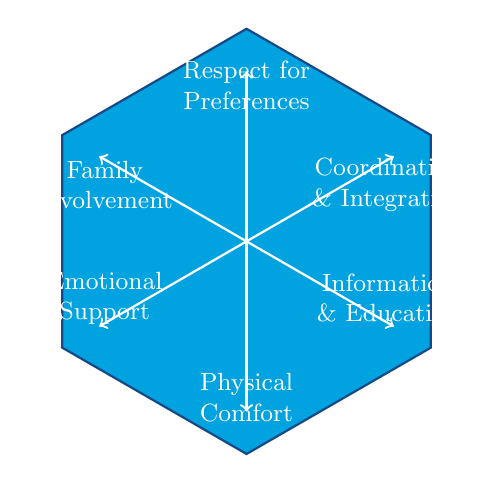
\begin{tikzpicture}[scale=0.9]
            % Central hexagon
            \draw[fill=darkblue, draw=none] (0,0) circle (1.5cm);
            \node[white, font=\bfseries, align=center] at (0,0) {Patient-\\Centered\\Care};
            
            % Outer dimensions
            \draw[fill=accent, draw=darkblue, thick] (0,3) -- (2.6,1.5) -- (2.6,-1.5) -- (0,-3) -- (-2.6,-1.5) -- (-2.6,1.5) -- cycle;
            
            % Dimension labels
            \node[white, font=\small, align=center] at (0,2.2) {Respect for\\Preferences};
            \node[white, font=\small, align=center] at (2,0.8) {Coordination\\\& Integration};
            \node[white, font=\small, align=center] at (2,-0.8) {Information\\\& Education};
            \node[white, font=\small, align=center] at (0,-2.2) {Physical\\Comfort};
            \node[white, font=\small, align=center] at (-2,-0.8) {Emotional\\Support};
            \node[white, font=\small, align=center] at (-2,0.8) {Family\\Involvement};
            
            % Arrows
            \foreach \a in {30, 90, 150, 210, 270, 330} {
                \draw[->, thick, white] (0,0) -- (\a:2.4);
            }
        \end{tikzpicture}
    \end{center}
    
    \smallskip
    
    The Picker Institute's eight principles of patient-centered care provide a comprehensive framework for understanding what patients value most in their healthcare experience, many of which are directly influenced by digital transformation initiatives \cite{cleveland2019}.
\end{frame}

\begin{frame}{Patient-Centered Care and Health Equity}
    \begin{columns}
        \begin{column}{0.5\textwidth}
            \begin{block}{Equity Dimensions}
                \begin{itemize}
                    \item \textbf{Individualized care}: Tailoring to each patient's unique circumstances
                    \item \textbf{Cultural competence}: Respecting diverse backgrounds and beliefs
                    \item \textbf{Language accessibility}: Overcoming communication barriers
                    \item \textbf{Health literacy}: Matching information to comprehension levels
                    \item \textbf{Shared decision-making}: Collaborative rather than paternalistic
                \end{itemize}
            \end{block}
        \end{column}
        \begin{column}{0.5\textwidth}
            \begin{block}{The Equity Imperative}
                True patient-centered care must address the needs of all patients, including those from marginalized communities who may face barriers to accessing and engaging with healthcare services. Digital tools can either bridge or widen these equity gaps depending on implementation approach.
            \end{block}
        \end{column}
    \end{columns}
    
    \pause
    
    \begin{block}{The Intersection}
        Patient-centered care and health equity are interdependent concepts. Care that is centered on patient preferences but inaccessible to certain populations fails to achieve its fundamental purpose. Digital transformation must be evaluated through both lenses simultaneously \cite{schwartz2019}.
    \end{block}
\end{frame}

%=======================================================================
% SECTION 2: DIGITAL TRANSFORMATION IN HEALTHCARE
%=======================================================================
\section{Digital Transformation in Healthcare}

\begin{frame}{Defining Digital Transformation}
    \begin{block}{Conceptual Definition}
        Digital transformation in healthcare refers to the fundamental change in how healthcare organizations create and deliver value to patients through the strategic application of digital technologies, data, and new business models. It represents a shift from technology-as-tool to technology-as-enabler of entirely new ways of engaging with patients and delivering care \cite{topol2019}.
    \end{block}
    
    \pause
    
    \begin{itemize}
        \item \textbf{Not merely digitization}: Moving from paper to electronic is automation, not transformation
        \item \textbf{Data-driven decision-making}: Using information at the point of care and for system improvement
        \item \textbf{Patient empowerment}: Shifting from provider-centric to patient-partner models
        \item \textbf{New care delivery models}: Virtual care, remote monitoring, and decentralized services
        \item \textbf{Connected ecosystems}: Integration across providers, patients, and payers
    \end{itemize}
\end{frame}

\begin{frame}{The Digital Health Landscape}
    \begin{center}
        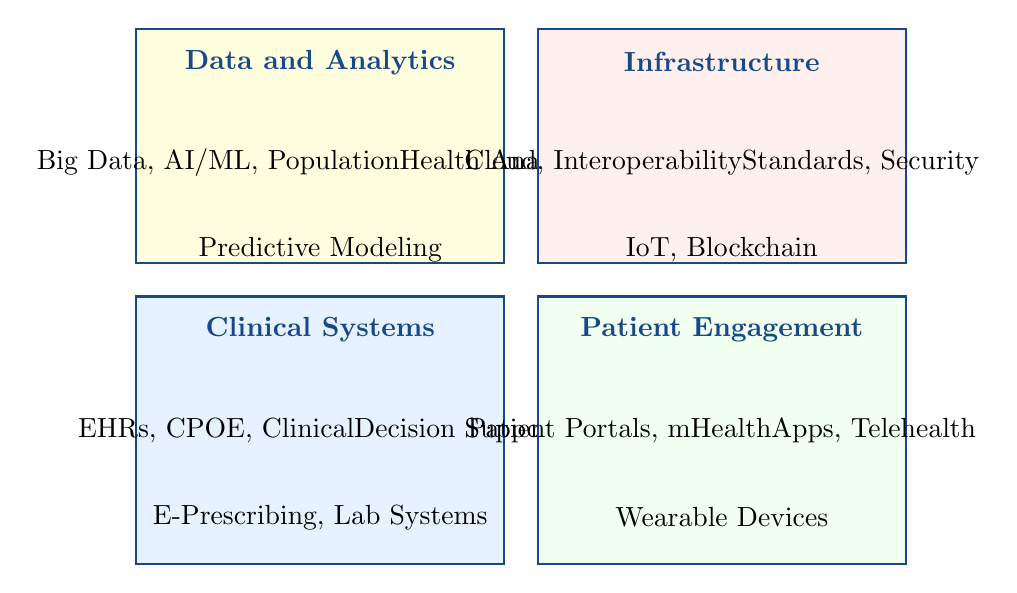
\begin{tikzpicture}[scale=0.85]
            % Four major categories
            \draw[fill=lightblue, draw=darkblue, thick] (0,0) rectangle (5.5,4);
            \node[darkblue, font=\bfseries] at (2.75,3.5) {Clinical Systems};
            \node[anchor=center] at (2.75,2) {EHRs, CPOE, Clinical\\Decision Support};
            \node[anchor=center] at (2.75,0.7) {E-Prescribing, Lab Systems};
            
            \draw[fill=lightgreen, draw=darkblue, thick] (6,0) rectangle (11.5,4);
            \node[darkblue, font=\bfseries] at (8.75,3.5) {Patient Engagement};
            \node[anchor=center] at (8.75,2) {Patient Portals, mHealth\\Apps, Telehealth};
            \node[anchor=center] at (8.75,0.7) {Wearable Devices};
            
            \draw[fill=lightyellow, draw=darkblue, thick] (0,4.5) rectangle (5.5,8);
            \node[darkblue, font=\bfseries] at (2.75,7.5) {Data and Analytics};
            \node[anchor=center] at (2.75,6) {Big Data, AI/ML, Population\\Health Analytics};
            \node[anchor=center] at (2.75,4.7) {Predictive Modeling};
            
            \draw[fill=lightred, draw=darkblue, thick] (6,4.5) rectangle (11.5,8);
            \node[darkblue, font=\bfseries] at (8.75,7.5) {Infrastructure};
            \node[anchor=center] at (8.75,6) {Cloud, Interoperability\\Standards, Security};
            \node[anchor=center] at (8.75,4.7) {IoT, Blockchain};
        \end{tikzpicture}
    \end{center}
    
    \smallskip
    
    Digital transformation encompasses multiple interacting domains, each of which contributes differently to patient-centered care. The integration and interoperability of these systems is critical for achieving comprehensive transformation \cite{agarwal2020}.
\end{frame}

\begin{frame}{Digital Transformation: Disruption and Evolution}
    \begin{columns}
        \begin{column}{0.5\textwidth}
            \begin{block}{Traditional Healthcare Model}
                \begin{itemize}
                    \item Provider-centric power dynamics
                    \item Episodic, facility-based encounters
                    \item Information locked in silos
                    \item Reactive rather than preventive
                    \item Limited patient agency
                    \item Provider as sole knowledge holder
                \end{itemize}
            \end{block}
        \end{column}
        \begin{column}{0.5\textwidth}
            \begin{block}{Digitally Transformed Model}
                \begin{itemize}
                    \item Patient-partnered care relationships
                    \item Continuous, distributed care delivery
                    \item Data liquid across boundaries
                    \item Proactive and predictive approaches
                    \item Empowered health consumers
                    \item Shared knowledge ecosystem
                \end{itemize}
            \end{block}
        \end{column}
    \end{columns}
    
    \pause
    
    \begin{block}{The Paradigm Shift}
        Digital transformation represents not just technological change but a fundamental restructuring of the patient-provider relationship and the very nature of healthcare delivery. The degree to which this transformation serves patient-centered ideals depends on deliberate design choices and governance frameworks.
    \end{block}
\end{frame}

%=======================================================================
% SECTION 3: KEY DIGITAL TOOLS AND TECHNOLOGIES
%=======================================================================
\section{Key Digital Tools and Technologies}

\begin{frame}{Electronic Health Records and Patient Portals}
    \begin{columns}
        \begin{column}{0.5\textwidth}
            \begin{block}{EHR Contributions to PCC}
                \begin{itemize}
                    \item Longitudinal patient history accessible to all providers
                    \item Clinical decision support promoting evidence-based care
                    \item Care coordination through shared information
                    \item Reduced duplicate testing and procedures
                    \item Automated safety alerts and reminders
                    \item Data infrastructure for population health
                \end{itemize}
            \end{block}
        \end{column}
        \begin{column}{0.5\textwidth}
            \begin{block}{Patient Portal Functions}
                \begin{itemize}
                    \item Secure messaging with care teams
                    \item Appointment scheduling and reminders
                    \item Access to test results and clinical notes
                    \item Medication refill requests
                    \item Health education resources
                    \item Pre-visit preparation tools
                    \item Care plan access and tracking
                \end{itemize}
            \end{block}
        \end{column}
    \end{columns}
    
    \pause
    
    \begin{block}{OpenNotes Movement}
        The OpenNotes initiative, now adopted by over 250 million patients, demonstrates how sharing clinical notes with patients can enhance understanding, trust, and engagement. Research shows improved medication adherence and patient satisfaction without increasing clinician workload \cite{bloom2019}.
    \end{block}
\end{frame}

\begin{frame}{Telemedicine and mHealth}
    \begin{center}
        \begin{tabular}{@{}lp{6cm}@{}}
            \toprule
            \textbf{Modality} & \textbf{Patient-Centered Contributions} \\
            \midrule
            \textbf{Video Consultations} & Convenience, reduced travel burden, visual assessment, personal connection \\
            \textbf{Store-and-Forward} & Asynchronous specialist access, record sharing \\
            \textbf{mHealth Apps} & Symptom tracking, health education, behavior change support \\
            \textbf{SMS Reminders} & Medication adherence, appointment attendance, preventive behaviors \\
            \textbf{Chatbots} & 24/7 information access, triage guidance, mental health support \\
            \textbf{Community Health Worker Tools} & Extended reach to underserved populations \\
            \bottomrule
        \end{tabular}
    \end{center}
    
    \pause
    
    \begin{block}{COVID-19 Acceleration}
        The pandemic catalyzed a decade of telemedicine adoption in months, demonstrating both the potential and limitations of virtual care. While telehealth improved access for many, it also revealed the digital divide affecting populations most in need of healthcare services \cite{hollander2020}.
    \end{block}
\end{frame}

\begin{frame}{Wearable Devices and Remote Patient Monitoring}
    \begin{columns}
        \begin{column}{0.5\textwidth}
            \begin{block}{Consumer Wearables}
                \begin{itemize}
                    \item Activity and step counting
                    \item Heart rate monitoring
                    \item Sleep tracking
                    \item ECG capabilities
                    \item Blood oxygen saturation
                    \item Menstrual cycle tracking
                \end{itemize}
            \end{block}
        \end{column}
        \begin{column}{0.5\textwidth}
            \begin{block}{Clinical Remote Monitoring}
                \begin{itemize}
                    \item Continuous glucose monitoring (CGM)
                    \item Remote cardiac telemetry
                    \item Blood pressure monitoring
                    \item Weight tracking for heart failure
                    \item Pulmonary function monitoring
                    \item Medication adherence monitoring
                \end{itemize}
            \end{block}
        \end{column}
    \end{columns}
    
    \pause
    
    \begin{block}{Value for Patient-Centered Care}
        Remote monitoring enables care to extend beyond facility walls, supporting aging in place, chronic disease management, and early intervention. However, data overload, alert fatigue, and integration challenges with clinical workflows remain significant barriers to realizing patient-centered benefits \cite{inan2020}.
    \end{block}
\end{frame}

\begin{frame}{AI-Assisted Clinical Decision Support}
    \begin{center}
        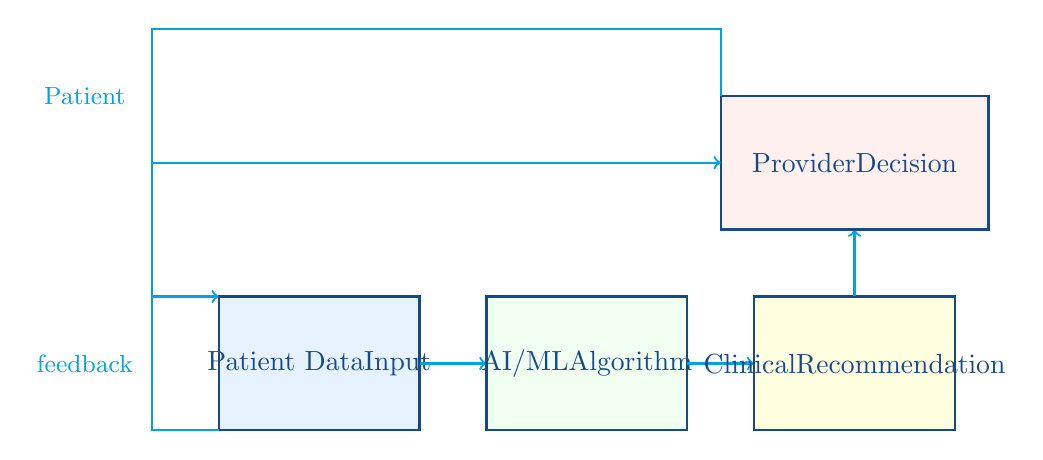
\begin{tikzpicture}[scale=0.85]
            % CDS workflow
            \draw[fill=lightblue, draw=darkblue, thick] (0,0) rectangle (3,2);
            \node[darkblue] at (1.5,1) {Patient Data\\Input};
            
            \draw[->, thick, accent] (3,1) -- (4,1);
            
            \draw[fill=lightgreen, draw=darkblue, thick] (4,0) rectangle (7,2);
            \node[darkblue] at (5.5,1) {AI/ML\\Algorithm};
            
            \draw[->, thick, accent] (7,1) -- (8,1);
            
            \draw[fill=lightyellow, draw=darkblue, thick] (8,0) rectangle (11,2);
            \node[darkblue] at (9.5,1) {Clinical\\Recommendation};
            
            \draw[->, thick, accent] (9.5,2) -- (9.5,3);
            
            \draw[fill=lightred, draw=darkblue, thick] (7.5,3) rectangle (11.5,5);
            \node[darkblue] at (9.5,4) {Provider\\Decision};
            
            % Patient loop
            \draw[->, thick, accent] (0,0) -- (-1,0) -- (-1,4) -- (7.5,4);
            \draw[->, thick, accent] (7.5,5) -- (7.5,6) -- (-1,6) -- (-1,2) -- (0,2);
            \node[accent, font=\small] at (-2,5) {Patient};
            \node[accent, font=\small] at (-2,1) {feedback};
        \end{tikzpicture}
    \end{center}
    
    \smallskip
    
    AI-assisted CDS ranges from drug interaction alerts to complex predictions about patient deterioration. When well-designed, CDS can reduce diagnostic errors, support evidence-based decisions, and free clinician time for patient interaction—potentially enhancing rather than replacing the human elements of care \cite{rajkomar2018}.
\end{frame}

%=======================================================================
% SECTION 4: DONABEDIAN'S MODEL APPLICATION
%=======================================================================
\section{Applying Donabedian's Model}

\begin{frame}{Donabedian's Structure-Process-Outcome Framework}
    \begin{block}{The Framework}
        Avedis Donabedian's quality framework, originally developed in 1966, remains foundational for evaluating healthcare interventions. The framework posits that healthcare quality can be assessed through three interrelated dimensions: the settings in which care occurs (structure), the activities that constitute care (process), and the results of care (outcomes) \cite{donabedian1988}.
    \end{block}
    
    \pause
    
    \begin{itemize}
        \item \textbf{Structure}: Physical facilities, equipment, human resources, organizational characteristics
        \item \textbf{Process}: What is actually done in giving and receiving care—technical and interpersonal dimensions
        \item \textbf{Outcome}: Changes in health status, knowledge, behavior, and patient satisfaction
    \end{itemize}
\end{frame}

\begin{frame}{Digital Transformation: Structure}
    \begin{center}
        \begin{tabular}{@{}lp{6cm}@{}}
            \toprule
            \textbf{Structural Element} & \textbf{Digital Transformation Impact} \\
            \midrule
            \textbf{Facilities} & Cloud-based systems reduce on-premise IT infrastructure needs; enables distributed care settings \\
            \textbf{Equipment} & Integration of medical devices with EHRs; proliferation of patient-owned devices \\
            \textbf{Human Resources} & Requires new roles (CMIO, data scientists, informatics specialists); workforce training demands \\
            \textbf{Organizational} & Flattened hierarchies; data-driven governance; cross-functional teams \\
            \textbf{Information Systems} & Electronic health records, data warehouses, interoperability infrastructure \\
            \bottomrule
        \end{tabular}
    \end{center}
    
    \pause
    
    \begin{block}{Structural Readiness}
        Organizations with strong IT infrastructure, governance frameworks, and workforce capacity are better positioned to leverage digital tools for patient-centered care. Structural deficiencies in any area can undermine digital transformation efforts regardless of technology sophistication.
    \end{block}
\end{frame}

\begin{frame}{Digital Transformation: Process}
    \begin{columns}
        \begin{column}{0.5\textwidth}
            \begin{block}{Technical Processes}
                \begin{itemize}
                    \item Order entry and results review
                    \item Clinical documentation and coding
                    \item Care coordination and handoffs
                    \item Population health management
                    \item Quality measurement and reporting
                    \item Supply chain and logistics
                \end{itemize}
            \end{block}
        \end{column}
        \begin{column}{0.5\textwidth}
            \begin{block}{Interpersonal Processes}
                \begin{itemize}
                    \item Patient-provider communication
                    \item Shared decision-making
                    \item Education and counseling
                    \item Care planning and goal-setting
                    \item Family engagement and involvement
                    \item Cultural sensitivity in care delivery
                \end{itemize}
            \end{block}
        \end{column}
    \end{columns}
    
    \pause
    
    \begin{block}{The Process Paradox}
        Digital tools can both enhance and undermine interpersonal processes. While messaging platforms and patient portals facilitate communication, excessive documentation requirements and alert fatigue can detract from face-to-face patient interaction. The balance depends on deliberate design and implementation choices \cite{street2019}.
    \end{block}
\end{frame}

\begin{frame}{Digital Transformation: Outcomes}
    \begin{center}
        \begin{tabular}{@{}lp{6cm}@{}}
            \toprule
            \textbf{Outcome Category} & \textbf{Potential Digital Contributions} \\
            \midrule
            \textbf{Clinical Outcomes} & Reduced errors, improved adherence, early intervention, chronic disease management \\
            \textbf{Patient Experience} & Convenience, communication, access, information, control \\
            \textbf{Patient Knowledge} & Health literacy, understanding of conditions, treatment options \\
            \textbf{Behavior Change} & Lifestyle modification, preventive behaviors, self-management \\
            \textbf{Provider Experience} & Burnout, satisfaction, efficiency, professional development \\
            \textbf{Population Health} & Surveillance, prevention, equity, cost sustainability \\
            \bottomrule
        \end{tabular}
    \end{center}
    
    \pause
    
    \begin{block}{Outcome Measurement Challenges}
        While process measures often show clear improvements with digital tools, linking technology interventions directly to health outcomes remains methodologically challenging. Patient-centered outcomes including experience, quality of life, and goal achievement are particularly important but difficult to attribute to specific digital interventions \cite{friedman2019}.
    \end{block}
\end{frame}

%=======================================================================
% SECTION 5: PATIENT ENGAGEMENT AND EMPOWERMENT
%=======================================================================
\section{Impact on Patient Engagement and Empowerment}

\begin{frame}{Defining Patient Engagement}
    \begin{columns}
        \begin{column}{0.5\textwidth}
            \begin{block}{Levels of Engagement}
                \begin{itemize}
                    \item \textbf{Compliance}: Following provider instructions
                    \item \textbf{Adherence}: Sustained engagement with treatment plans
                    \item \textbf{Involvement}: Active participation in care decisions
                    \item \textbf{Partnership}: Collaborative relationship with providers
                    \item \textbf{Self-management}: Independent management of health
                    \item \textbf{Activation}: Understanding and exercising health rights
                \end{itemize}
            \end{block}
        \end{column}
        \begin{column}{0.5\textwidth}
            \begin{block}{Patient Activation Measure (PAM)}
                The PAM assesses patient knowledge, skills, and confidence for health self-management. Research consistently shows that higher activation correlates with better outcomes, lower costs, and greater satisfaction. Digital tools may enhance or undermine activation depending on design and implementation.
            \end{block}
        \end{column}
    \end{columns}
    
    \pause
    
    \begin{block}{Digital Engagement Mechanisms}
        Patient portals, mHealth apps, wearable devices, and social media communities can support engagement at multiple levels, but engagement with technology does not automatically translate to engagement with health. The distinction between clicking buttons and meaningful health behavior change is critical \cite{ojen2019}.
    \end{block}
\end{frame}

\begin{frame}{Patient Empowerment Through Information}
    \begin{center}
        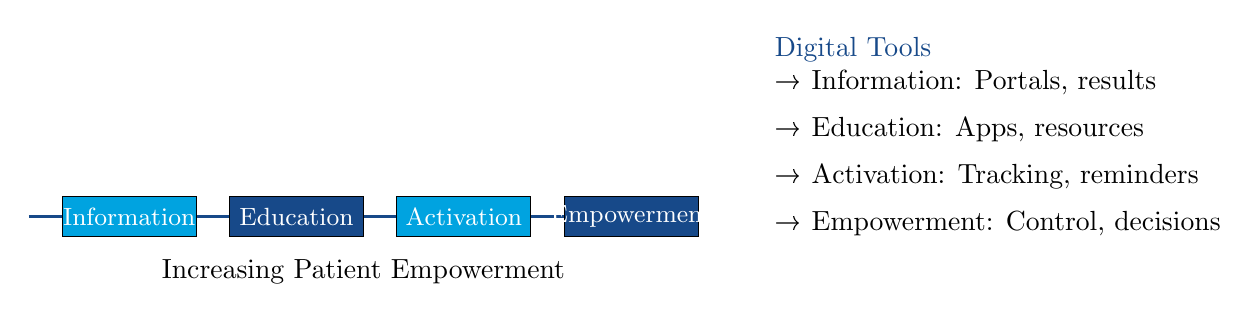
\begin{tikzpicture}[scale=0.85]
            % Empowerment spectrum
            \draw[->, thick, darkblue] (0,0) -- (10,0);
            \node[anchor=north] at (5,-0.5) {Increasing Patient Empowerment};
            
            % Stages
            \draw[fill=accent] (0.5,-0.3) rectangle (2.5,0.3);
            \node[white, font=\small] at (1.5,0) {Information};
            
            \draw[fill=darkblue] (3,-0.3) rectangle (5,0.3);
            \node[white, font=\small] at (4,0) {Education};
            
            \draw[fill=accent] (5.5,-0.3) rectangle (7.5,0.3);
            \node[white, font=\small] at (6.5,0) {Activation};
            
            \draw[fill=darkblue] (8,-0.3) rectangle (10,0.3);
            \node[white, font=\small] at (9,0) {Empowerment};
            
            % Digital tools supporting each stage
            \node[darkblue, anchor=west] at (11,2.5) {Digital Tools};
            \node[anchor=west] at (11,2) {→ Information: Portals, results};
            \node[anchor=west] at (11,1.3) {→ Education: Apps, resources};
            \node[anchor=west] at (11,0.6) {→ Activation: Tracking, reminders};
            \node[anchor=west] at (11,-0.1) {→ Empowerment: Control, decisions};
        \end{tikzpicture}
    \end{center}
    
    \smallskip
    
    Digital tools can facilitate patient empowerment by providing information, enabling tracking, supporting self-management, and facilitating communication with providers. However, the degree of empowerment depends on whether tools are designed with patient agency as a primary goal rather than a byproduct \cite{vanhoudenhoven2019}.
\end{frame}

\begin{frame}{Barriers to Patient Engagement}
    \begin{columns}
        \begin{column}{0.5\textwidth}
            \begin{block}{Patient-Level Barriers}
                \begin{itemize}
                    \item Digital literacy and access gaps
                    \item Health literacy limitations
                    \item Cognitive burden of illness
                    \item Competing life demands
                    \item Mistrust of technology or providers
                    \item Cultural and language barriers
                \end{itemize}
            \end{block}
        \end{column}
        \begin{column}{0.5\textwidth}
            \begin{block}{System-Level Barriers}
                \begin{itemize}
                    \item Fragmented, non-integrated systems
                    \item Usability problems and poor design
                    \item Limited functionality (write vs. read-only)
                    \item Lack of personalization and relevance
                    \item Privacy concerns and data fears
                    \item Provider resistance to patient access
                \end{itemize}
            \end{block}
        \end{column}
    \end{columns}
    
    \pause
    
    \begin{block}{The Engagement Paradox}
        While digital tools theoretically enable greater patient engagement, those most likely to benefit—patients with chronic conditions, low health literacy, or limited access—may be least likely to engage with digital tools. Without deliberate attention to these barriers, digital patient engagement may worsen rather than improve health equity \cite{anthes2019}.
    \end{block}
\end{frame}

%=======================================================================
% SECTION 6: QUALITY AND CONTINUITY OF CARE
%=======================================================================
\section{Impact on Quality and Continuity of Care}

\begin{frame}{Digital Tools and Care Quality}
    \begin{center}
        \begin{tabular}{@{}lp{6cm}@{}}
            \toprule
            \textbf{Quality Dimension} & \textbf{Digital Enhancement} \\
            \midrule
            \textbf{Safety} & Drug interaction checking, allergy alerts, diagnostic support, error reduction \\
            \textbf{Effectiveness} & Evidence-based guidelines, clinical pathways, outcome tracking \\
            \textbf{Timeliness} & Reduced wait times, rapid result delivery, queue management \\
            \textbf{Efficiency} & Automated workflows, reduced duplication, resource optimization \\
            \textbf{Equity} & Expanded access, population segmentation, targeted outreach \\
            \bottomrule
        \end{tabular}
    \end{center}
    
    \pause
    
    \begin{block}{Quality by Design}
        Digital tools can enhance multiple dimensions of care quality, but this potential is only realized when systems are designed with quality as an explicit goal. Technology implemented without quality frameworks may create new inefficiencies and safety risks even while addressing others.
    \end{block}
\end{frame}

\begin{frame}{Continuity of Care in Digital Systems}
    \begin{columns}
        \begin{column}{0.5\textwidth}
            \begin{block}{Information Continuity}
                \begin{itemize}
                    \item Longitudinal EHR accessible across settings
                    \item Structured data enabling interpretation
                    \item Care plan sharing and synchronization
                    \item Medication reconciliation support
                    \item Allergy and alert sharing
                \end{itemize}
            \end{block}
        \end{column}
        \begin{column}{0.5\textwidth}
            \begin{block}{Relational Continuity}
                \begin{itemize}
                    \item Patient portal maintaining connection between visits
                    \item Secure messaging with established providers
                    \item Care team identification and access
                    \item Virtual visit options maintaining relationships
                    \item Family and caregiver access and involvement
                \end{itemize}
            \end{block}
        \end{column}
    \end{columns}
    
    \pause
    
    \begin{block}{The Continuity Challenge}
        While digital systems can enhance information continuity, the fragmentation of healthcare across multiple organizations and platforms often undermines relational continuity. Patients may have excellent information flow but never see the same provider twice. True patient-centered care requires addressing both dimensions simultaneously \cite{vanallen2018}.
    \end{block}
\end{frame}

\begin{frame}{The Quality-Time Paradox}
    \begin{center}
        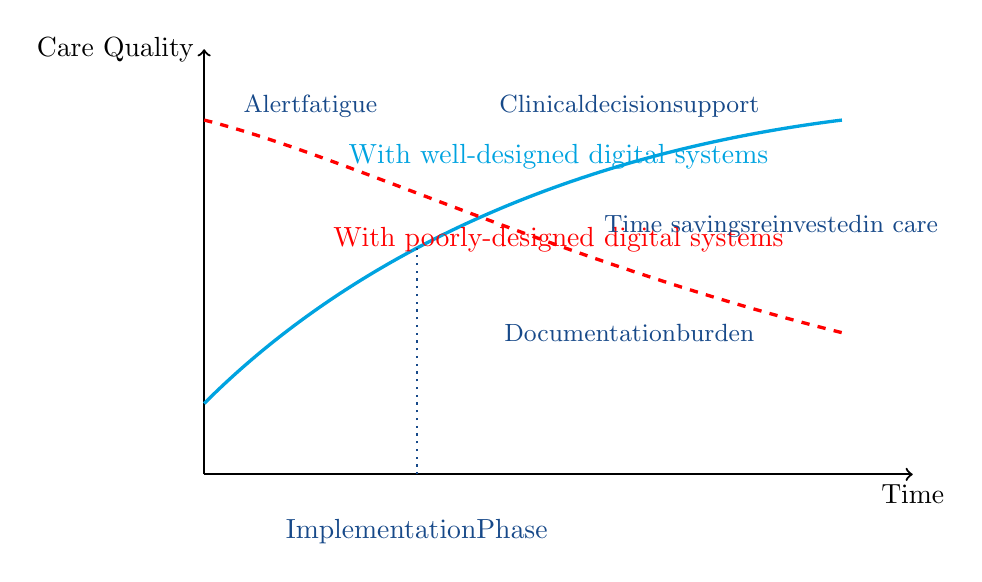
\begin{tikzpicture}[scale=0.9]
            % Two axes
            \draw[->, thick] (0,0) -- (10,0) node[below] {Time};
            \draw[->, thick] (0,0) -- (0,6) node[left] {Care Quality};
            
            % Curves
            \draw[very thick, accent] (0,1) .. controls (2,3) and (5,4.5) .. (9,5);
            \draw[very thick, red, dashed] (0,5) .. controls (2,4.5) and (5,3) .. (9,2);
            
            % Labels
            \node[accent, anchor=north] at (5,4.8) {With well-designed digital systems};
            \node[red, anchor=south] at (5,3) {With poorly-designed digital systems};
            
            % Critical points
            \draw[dotted, thick, darkblue] (3,0) -- (3,3.2);
            \node[darkblue, anchor=north] at (3,-0.5) {Implementation\\Phase};
            
            \node[darkblue, font=\small] at (6,2) {Documentation\\burden};
            \node[darkblue, font=\small] at (6,5.2) {Clinical\\decision\\support};
            
            \node[darkblue, font=\small] at (1.5,5.2) {Alert\\fatigue};
            \node[darkblue, font=\small] at (8,3.5) {Time savings\\reinvested\\in care};
        \end{tikzpicture}
    \end{center}
    
    \smallskip
    
    The relationship between digital tools and care quality is not linear. Initial implementation often reduces quality as providers adapt, but long-term outcomes depend on system design, training, and continuous optimization. The quality curve can go up or down depending on implementation approach \cite{shah2019}.
\end{frame}

%=======================================================================
% SECTION 7: ACCESS AND EQUITY
%=======================================================================
\section{Impact on Access and Equity}

\begin{frame}{Digital Enhancement of Access}
    \begin{center}
        \begin{tikzpicture}[scale=0.85]
            % Access dimensions
            \draw[fill=lightblue, draw=darkblue, thick] (0,0) rectangle (12,7);
            
            \node[darkblue, font=\bfseries, fontsize=14] at (6,6.3) {Digital Enhancement of Healthcare Access};
            
            % Geographic access
            \node[darkblue, font=\bfseries, anchor=east] at (3,5) {Geographic};
            \node[anchor=west] at (3.2,5) {Telehealth eliminates travel barriers; rural specialist access};
            
            % Temporal access
            \node[darkblue, font=\bfseries, anchor=east] at (3,4) {Temporal};
            \node[anchor=west] at (3.2,4) {24/7 portals and chatbots; async communication};
            
            % Financial access
            \node[darkblue, font=\bfseries, anchor=east] at (3,3) {Financial};
            \node[anchor=west] at (3.2,3) {Reduced indirect costs (travel, time off work)};
            
            % Informational access
            \node[darkblue, font=\bfseries, anchor=east] at (3,2) {Informational};
            \node[anchor=west] at (3.2,2) {Health education, symptom checking, provider information};
            
            % Cultural access
            \node[darkblue, font=\bfseries, anchor=east] at (3,1) {Cultural};
            \node[anchor=west] at (3.2,1) {Language options; anonymous health咨询};
            
            % Right side - barriers
            \draw[fill=lightred, draw=darkblue, thick] (7,1) rectangle (11.5,6);
            \node[darkblue, font=\bfseries] at (9.25,5.5) {Access Barriers};
            \node[anchor=center] at (9.25,4) {Digital divide (skills, devices,\\connectivity)};
            \node[anchor=center] at (9.25,2.5) {Privacy concerns limiting use};
            \node[anchor=center] at (9.25,1.2) {Technology not designed\\for all users};
        \end{tikzpicture}
    \end{center}
    
    \smallskip
    
    Digital tools can theoretically enhance all dimensions of access, but realizing this potential requires addressing the barriers that prevent some populations from benefiting. Access gains for the connected majority may be offset by exclusion of marginalized groups \cite{worldbank2019}.
\end{frame}

\begin{frame}{The Digital Divide and Health Equity}
    \begin{columns}
        \begin{column}{0.5\textwidth}
            \begin{block}{Dimensions of the Divide}
                \begin{itemize}
                    \item \textbf{Access divide}: Lack of devices, connectivity, or data plans
                    \item \textbf{Skills divide}: Digital literacy and health literacy limitations
                    \item \textbf{Usage divide}: Qualitative differences in how technology is used
                    \item \textbf{Outcome divide}: Differential health benefits from digital engagement
                \end{itemize}
            \end{block}
        \end{column}
        \begin{column}{0.5\textwidth}
            \begin{block}{Vulnerable Populations}
                \begin{itemize}
                    \item Elderly adults with limited technology exposure
                    \item Low-income individuals with device and data costs
                    \item Rural populations with connectivity gaps
                    \item Non-native language speakers
                    \item Persons with disabilities
                    \item Individuals with serious mental illness
                \end{itemize}
            \end{block}
        \end{column}
    \end{columns}
    
    \pause
    
    \begin{block}{Equity Implications}
        Research consistently shows that digital health interventions benefit populations with higher socioeconomic status and digital literacy first, potentially widening existing health inequities. Unless equity is deliberately prioritized, digital transformation may create a two-tiered healthcare system \cite{percival2019}.
    \end{block}
\end{frame}

\begin{frame}{Strategies for Digital Equity}
    \begin{center}
        \begin{tabular}{@{}lp{6cm}@{}}
            \toprule
            \textbf{Strategy} & \textbf{Approach} \\
            \midrule
            \textbf{Multimodal access} & Offering phone, video, in-person, and mail options simultaneously \\
            \textbf{Community access points} & Libraries, community centers, pharmacies as digital health hubs \\
            \textbf{Universal design} & Technology usable by people with varying abilities without adaptation \\
            \textbf{Offline functionality} & Systems that work without continuous connectivity \\
            \textbf{Digital navigators} & Trained personnel to assist with technology adoption \\
            \textbf{Equity monitoring} & Disaggregated data to identify and address disparities \\
            \bottomrule
        \end{tabular}
    \end{center}
    
    \pause
    
    \begin{block}{Beyond Digital-Only}
        The most equitable approach is to offer multiple access modalities, ensuring that digital tools complement rather than replace traditional access routes. Organizations committed to patient-centered care must resist the temptation to shift entirely to digital channels that exclude portions of their patient population.
    \end{block}
\end{frame}

%=======================================================================
% SECTION 8: ETHICAL, PRIVACY, AND DATA PROTECTION CONCERNS
%=======================================================================
\section{Ethical, Privacy, and Data Protection Concerns}

\begin{frame}{Ethical Considerations in Digital Health}
    \begin{columns}
        \begin{column}{0.5\textwidth}
            \begin{block}{Autonomy and Agency}
                \begin{itemize}
                    \item Informed consent for data collection and use
                    \item Transparency about algorithmic recommendations
                    \item Patient control over data sharing
                    \item Right to refuse digital services
                    \item Protection from manipulation (persuasive tech)
                \end{itemize}
            \end{block}
        \end{column}
        \begin{column}{0.5\textwidth}
            \begin{block}{Beneficence and Non-Maleficence}
                \begin{itemize}
                    \item Ensuring AI algorithms are validated and fair
                    \item Avoiding technology that increases anxiety
                    \item Protecting against diagnostic errors from CDS
                    \item Preventing surveillance and its psychological effects
                    \item Ensuring equitable access and outcomes
                \end{itemize}
            \end{block}
        \end{column}
    \end{columns}
    
    \pause
    
    \begin{block}{The Ethics Framework}
        Digital health interventions should be evaluated against standard biomedical ethics principles: respect for autonomy, beneficence, non-maleficence, and justice. Digital tools introduce new complexities—algorithmic opacity, data commodification, and surveillance potential—that require adapted ethical frameworks and governance mechanisms \cite{price2019}.
    \end{block}
\end{frame}

\begin{frame}{Privacy and Data Protection}
    \begin{center}
        \begin{tikzpicture}[scale=0.85]
            % Privacy threats
            \draw[fill=lightred, draw=darkblue, thick] (0,0) rectangle (12,7);
            
            \node[darkblue, font=\bfseries, fontsize=14] at (6,6.3) {Privacy Threats in Digital Health};
            
            % Threats
            \node[anchor=east] at (3,5) {\begin{tikzpicture}\draw[fill=darkblue] (0,0) circle (0.4);\end{tikzpicture}};
            \node[anchor=west] at (3.2,5) {Data breaches exposing sensitive health information};
            
            \node[anchor=east] at (3,4) {
\begin{tikzpicture}\draw[fill=darkblue] (0,0) circle (0.4);\end{tikzpicture}};
            \node[anchor=west] at (3.2,4) {Third-party data sharing for commercial purposes};
            
            \node[anchor=east] at (3,3) {
\begin{tikzpicture}\draw[fill=darkblue] (0,0) circle (0.4);\end{tikzpicture}};
            \node[anchor=west] at (3.2,3) {Re-identification of anonymized datasets};
            
            \node[anchor=east] at (3,2) {
\begin{tikzpicture}\draw[fill=darkblue] (0,0) circle (0.4);\end{tikzpicture}};
            \node[anchor=west] at (3.2,2) {Employer or insurer access to personal data};
            
            \node[anchor=east] at (3,1) {
\begin{tikzpicture}\draw[fill=darkblue] (0,0) circle (0.4);\end{tikzpicture}};
            \node[anchor=west] at (3.2,1) {Government surveillance and data retention};
            
            % Right side - protections
            \node[darkblue, font=\bfseries] at (9,5.5) {Protective Measures};
            \node[anchor=center] at (9,4) {Regulatory frameworks};
            \node[anchor=center] at (9,3) {Technical safeguards};
            \node[anchor=center] at (9,2) {Organizational policies};
            \node[anchor=center] at (9,1) {Patient controls};
        \end{tikzpicture}
    \end{center}
    
    \smallskip
    
    Health data is among the most sensitive personal information, and digital systems create unprecedented opportunities for collection, aggregation, and potential misuse. Trust in digital health depends on robust privacy protections that give patients meaningful control over their information \cite{cohen2018}.
\end{frame}

\begin{frame}{Data Protection Regulatory Landscape}
    \begin{columns}
        \begin{column}{0.5\textwidth}
            \begin{block}{Key Regulations}
                \begin{itemize}
                    \item \textbf{HIPAA (US)}: Sets baseline for health data protection
                    \item \textbf{GDPR (EU)}: Strongest privacy framework with explicit health data provisions
                    \item \textbf{HITECH Act}: Extends HIPAA to address technology
                    \item \textbf{21st Century Cures Act}: Promotes information blocking prohibition
                \end{itemize}
            \end{block}
        \end{column}
        \begin{column}{0.5\textwidth}
            \begin{block}{Emerging Challenges}
                \begin{itemize}
                    \item Consumer health data outside traditional regulations
                    \item Cross-border data flows and jurisdictional conflicts
                    \item AI and algorithmic decision-making opacity
                    \item Secondary use of clinical data for research
                    \item Genomic data and precision medicine implications
                \end{itemize}
            \end{block}
        \end{column}
    \end{columns}
    
    \pause
    
    \begin{block}{The Governance Gap}
                While regulatory frameworks have evolved, they often lag behind technological capabilities. Consumer health apps, wearable devices, and direct-to-consumer genetic testing frequently operate outside traditional healthcare regulations, leaving significant gaps in data protection that undermine patient trust and potentially patient-centered care \cite{vojinovic2019}.
    \end{block}
\end{frame}

\begin{frame}{Algorithmic Fairness and Bias}
    \begin{center}
        \begin{tabular}{@{}lp{6cm}@{}}
            \toprule
            \textbf{Bias Source} & \textbf{Impact on Patient-Centered Care} \\
            \midrule
            \textbf{Training data bias} & Algorithms perform poorly for underrepresented groups \\
            \textbf{Label bias} & Historical inequities embedded in prediction targets \\
            \textbf{Feature bias} & Proxies for race/ethnicity creating discrimination \\
            \textbf{Deployment bias} & Algorithms validated in one context applied elsewhere \\
            \textbf{Feedback loops} & Biased predictions reinforce existing inequities \\
            \bottomrule
        \end{tabular}
    \end{center}
    
    \pause
    
    \begin{block}{The Fairness Imperative}
        AI systems used in healthcare can perpetuate or amplify existing biases if not carefully designed and monitored. Patient-centered care requires algorithmic fairness as a core requirement, with diverse development teams, bias testing across populations, and ongoing monitoring for disparate impact \cite{obeng2019}.
    \end{block}
\end{frame}

%=======================================================================
% SECTION 9: BALANCED ASSESSMENT
%=======================================================================
\section{Balanced Assessment: Benefits and Risks}

\begin{frame}{Benefits of Digital Transformation for PCC}
    \begin{columns}
        \begin{column}{0.5\textwidth}
            \begin{block}{Enhanced Patient Experience}
                \begin{itemize}
                    \item Convenience of digital access
                    \item Enhanced communication channels
                    \item Access to personal health information
                    \item Support for self-management
                    \item Personalized education and resources
                    \item Reduced administrative burden
                \end{itemize}
            \end{block}
        \end{column}
        \begin{column}{0.5\textwidth}
            \begin{block}{Improved Care Quality}
                \begin{itemize}
                    \item Reduced medical errors
                    \item Evidence-based clinical decision support
                    \item Enhanced care coordination
                    \item Early intervention through monitoring
                    \item Population health management
                    \item Safety surveillance and alerts
                \end{itemize}
            \end{block}
        \end{column}
    \end{columns}
    
    \pause
    
    \begin{block}{Systematic Evidence}
                Systematic reviews consistently find that patient-facing digital interventions improve patient satisfaction, self-management, and some clinical outcomes. The magnitude of benefit varies considerably based on implementation quality, patient characteristics, and the specific intervention \cite{flodgren2015}.
    \end{block}
\end{frame}

\begin{frame}{Risks and Unintended Consequences}
    \begin{columns}
        \begin{column}{0.5\textwidth}
            \begin{block}{Patient-Level Risks}
                \begin{itemize}
                    \item Privacy violations and data misuse
                    \item Digital exclusion of vulnerable populations
                    \item Technology-induced anxiety and overwhelm
                    \item Misinformation from unreliable digital sources
                    \item Reduced human interaction in care
                    \item Algorithmic discrimination
                \end{itemize}
            \end{block}
        \end{column}
        \begin{column}{0.5\textwidth}
            \begin{block}{System-Level Risks}
                \begin{itemize}
                    \item Alert fatigue and desensitization
                    \item Documentation burden reducing face time
                    \item System fragmentation and information blocking
                    \item Vendor lock-in and interoperability failures
                    \item Cybersecurity vulnerabilities
                    \item Sustainability and cost concerns
                \end{itemize}
            \end{block}
        \end{column}
    \end{columns}
    
    \pause
    
    \begin{block}{The Need for Vigilance}
        The risks of digital transformation are not merely theoretical—they manifest in patient harm, eroded trust, and health inequities. Patient-centered care requires proactive identification and mitigation of these risks rather than uncritical technology adoption \cite{vernon2019}.
    \end{block}
\end{frame}

\begin{frame}{The Balance Matrix}
    \begin{center}
        \begin{tabular}{@{}lcc@{}}
            \toprule
            \textbf{Dimension} & \textbf{Potential Benefit} & \textbf{Potential Risk} \\
            \midrule
            Access & Geographic reach expanded & Digital divide exacerbated \\
            Communication & Multiple channels enabled & Fragmented conversations \\
            Information & Patient data access & Privacy vulnerabilities \\
            Self-management & Tracking and reminders & Measurement burden \\
            Clinical care & Decision support & Alert fatigue, errors \\
            Relationship & Virtual connection options & Reduced in-person contact \\
            Equity & Tailored interventions & Bias and discrimination \\
            Trust & Transparency tools & Surveillance concerns \\
            \bottomrule
        \end{tabular}
    \end{center}
    
    \pause
    
    \begin{block}{Context-Dependent Assessment}
        The balance of benefits and risks varies by patient population, clinical context, implementation approach, and organizational culture. There is no universal answer to whether digital transformation serves patient-centered care—it depends on how technologies are designed, implemented, and governed.
    \end{block}
\end{frame}

%=======================================================================
% SECTION 10: CONCLUSIONS AND IMPLICATIONS
%=======================================================================
\section{Conclusions and Implications}

\begin{frame}{Summary: Digital Transformation and PCC}
    \begin{enumerate}
        \item \textbf{Enabling but not sufficient}: Digital tools can enhance patient-centered care but cannot substitute for fundamental relational and systemic requirements
        \item \textbf{Design matters enormously}: Technology designed with patient agency as a core principle produces different outcomes than technology designed primarily for efficiency or data extraction
        \item \textbf{Equity is essential}: Without deliberate equity focus, digital transformation risks widening health disparities
        \item \textbf{Privacy enables trust}: Robust data protection is foundational for patient willingness to engage with digital tools
        \item \textbf{Human in the loop}: Technology should augment, not replace, human connection in healthcare
        \item \textbf{Continuous evaluation}: Patient-centered outcomes must be systematically measured and used to guide ongoing improvement
    \end{enumerate}
    
    \pause
    
    \begin{block}{The Synthesis}
        Digital transformation represents both an opportunity and an obligation for healthcare organizations committed to patient-centered care. The technology itself is morally neutral—it is the purposes to which it is put and the values that guide its implementation that determine whether it serves or undermines patient-centeredness.
    \end{block}
\end{frame}

\begin{frame}{Policy and Practice Implications}
    \begin{columns}
        \begin{column}{0.5\textwidth}
            \begin{block}{For Healthcare Organizations}
                \begin{itemize}
                    \item Center patient voices in technology design
                    \item Maintain non-digital access options
                    \item Invest in digital literacy for patients and staff
                    \item Monitor outcomes by patient characteristics
                    \item Build robust data governance frameworks
                    \item Evaluate technology against patient-centered goals
                \end{itemize}
            \end{block}
        \end{column}
        \begin{column}{0.5\textwidth}
            \begin{block}{For Policymakers}
                \begin{itemize}
                    \item Extend privacy protections to all health data
                    \item Require algorithmic fairness assessment
                    \item Fund digital equity initiatives
                    \item Support research on patient-centered outcomes
                    \item Create regulatory sandboxes for innovation
                    \item Coordinate across sectors for population health
                \end{itemize}
            \end{block}
        \end{column}
    \end{columns}
    
    \pause
    
    \begin{block}{For Technology Developers}
                Companies creating digital health tools must move beyond minimum viable products to evidence-based, patient-centered solutions that demonstrate meaningful health impact. The valley of death between pilot and implementation must be bridged with rigorous evaluation and continuous improvement.
    \end{block}
\end{frame}

\begin{frame}{Final Reflection}
    \begin{center}
        \begin{quotation}
            \textit{``The measure of digital transformation's success is not how many patients use our portal or app, but whether their health improves, their experience strengthens, and their values are honored. Technology is in service to people, never the reverse.''}
        \end{quotation}
    \end{center}
    
    \bigskip
    
    The opportunity before us is to harness digital transformation in service of the timeless goals of healthcare: healing, comfort, dignity, and partnership. The risk is that we become so enamored with technology that we lose sight of these purposes. Patient-centered care demands that we hold both possibilities in mind as we navigate this transformation.
    
    \bigskip
    
    \hfill \textbf{Thank you. Questions?}
\end{frame}

%=======================================================================
% REFERENCES
%=======================================================================
\section{References}
\begin{frame}[allowframebreaks]{References}
    \begin{thebibliography}{99}
        
        \bibitem{agarwal2020}
        Agarwal, R., et al. (2020). The digital transformation of healthcare: Current status and the road ahead. \textit{Information Systems Research}, 31(4), 1154-1172.
        
        \bibitem{anthes2019}
        Anthes, E. (2019). Digital health: The battle for the user's attention. \textit{Nature}, 573(7773), 122-124.
        
        \bibitem{bloom2019}
        Bloom, S., et al. (2019). OpenNotes and patient safety: A systematic review. \textit{Journal of General Internal Medicine}, 34(10), 2075-2082.
        
        \bibitem{cleveland2019}
        Cleveland, K.A., et al. (2019). Patient-centered care: A conceptual model and review of the literature. \textit{Health Care Management Review}, 44(4), 312-322.
        
        \bibitem{cohen2018}
        Cohen, I.G. (2018). \textit{Health Privacy in the Digital Age}. New York: NYU School of Law.
        
        \bibitem{donabedian1988}
        Donabedian, A. (1988). The quality of care: How can it be assessed? \textit{JAMA}, 260(12), 1743-1748.
        
        \bibitem{flodgren2015}
        Flodgren, G., et al. (2015). Interactive telemedicine: Effects on professional practice and health care outcomes. \textit{Cochrane Database of Systematic Reviews}, 9, CD002098.
        
        \bibitem{friedman2019}
        Friedman, C.P., et al. (2019). A road map for academic health systems to sustain precision innovation and population health improvement. \textit{Academic Medicine}, 94(9), 1293-1298.
        
        \bibitem{hollander2020}
        Hollander, J.E., \& Carr, B.G. (2020). Virtually perfect? Telemedicine for Covid-19. \textit{New England Journal of Medicine}, 382(18), 1679-1681.
        
        \bibitem{IOM2001}
        Institute of Medicine. (2001). \textit{Crossing the Quality Chasm: A New Health System for the 21st Century}. Washington, DC: National Academy Press.
        
        \bibitem{inan2020}
        Inan, O.T., et al. (2020). Digitizing the clinical encounter. \textit{Nature Medicine}, 26(12), 1815-1818.
        
        \bibitem{ojen2019}
        Ojen, R., et al. (2019). Conceptualizing patient engagement in health care: A scoping review of the literature. \textit{Journal of General Internal Medicine}, 34(12), 2781-2790.
        
        \bibitem{percival2019}
        Percival, J., et al. (2019). The digital divide and health disparities. \textit{Journal of Medical Internet Research}, 21(6), e12841.
        
        \bibitem{price2019}
        Price, W.N., \& Cohen, I.G. (2019). Privacy in the age of medical big data. \textit{Nature Medicine}, 25(1), 37-43.
        
        \bibitem{rajkomar2018}
        Rajkomar, A., et al. (2018). Scalable and accurate deep learning with electronic health records. \textit{NPJ Digital Medicine}, 1(1), 18.
        
        \bibitem{schwartz2019}
        Schwartz, P.H., et al. (2019). Patient-centered digital health. \textit{Journal of Medical Ethics}, 45(10), 679-683.
        
        \bibitem{shah2019}
        Shah, N.R., et al. (2019). Health information technology: A year in review. \textit{Journal of the American Medical Informatics Association}, 26(11), 1275-1280.
        
        \bibitem{street2019}
        Street, R.L., et al. (2019). How does communication heal? Pathways linking clinician-patient communication to health outcomes. \textit{Patient Education and Counseling}, 102(3), 395-401.
        
        \bibitem{topol2019}
        Topol, E. (2019). \textit{Deep Medicine: How AI Can Make Healthcare Human Again}. New York: Basic Books.
        
        \bibitem{vanallen2018}
        Van Allen, T.N., et al. (2018). Physician perspectives on long-term patient relationships. \textit{Journal of General Internal Medicine}, 33(8), 1295-1301.
        
        \bibitem{vanhoudenhoven2019}
        Van Houdenhoven, M., et al. (2019). Patient empowerment through digital health. \textit{International Journal of Medical Informatics}, 127, 21-27.
        
        \bibitem{vernon2019}
        Vernon, J., et al. (2019). The unintended consequences of digital health. \textit{Journal of Medical Ethics}, 45(7), 417-421.
        
        \bibitem{vojinovic2019}
        Vojinovic, D., et al. (2019). Data protection in health research: A systematic review. \textit{International Journal of Medical Informatics}, 126, 122-131.
        
        \bibitem{worldbank2019}
        World Bank. (2019). \textit{World Development Report 2019: The Changing Nature of Work}. Washington, DC: World Bank Group.
        
    \end{thebibliography}
\end{frame}

\end{document}
